% !TEX TS-program = XeLaTeX
% use the following command:
% all document files must be coded in UTF-8
\documentclass[spanish]{textolivre}
% build HTML with: make4ht -e build.lua -c textolivre.cfg -x -u article "fn-in,svg,pic-align"

\journalname{Texto Livre}
\thevolume{16}
%\thenumber{1} % old template
\theyear{2023}
\receiveddate{\DTMdisplaydate{2022}{11}{21}{-1}} % YYYY MM DD
\accepteddate{\DTMdisplaydate{2023}{1}{3}{-1}}
\publisheddate{\DTMdisplaydate{2023}{1}{19}{-1}}
\corrauthor{María Victoria López-Pérez}
\articledoi{10.1590/1983-3652.2023.41879}
%\articleid{NNNN} % if the article ID is not the last 5 numbers of its DOI, provide it using \articleid{} commmand 
% list of available sesscions in the journal: articles, dossier, reports, essays, reviews, interviews, editorial
\articlesessionname{dossier}
\runningauthor{López-Pérez y Bobadilla-Pérez} 
%\editorname{Leonardo Araújo} % old template
\sectioneditorname{Hugo Heredia Ponce}
\layouteditorname{Daniervelin Pereira}

\title{Alfabetización multimodal y plurialfabetización en Educación Primaria a través de la narrativa transmediática \textit{El niño, el topo, el zorro y el caballo}, de Charlie Mackesy}
\othertitle{Letramento multimodal e pluriletramentos na educação básica por meio da narrativa transmídia \textit{El niño, el topo, el zorro y el caballo}, de Charlie Mackesy}
\othertitle{Multimodal literacy and pluriliteracy in the Primary School classroom through a transmedia narrative \textit{El niño, el topo, el zorro y el caballo}, by Charlie Mackesy}
% if there is a third language title, add here:
%\othertitle{Artikelvorlage zur Einreichung beim Texto Livre Journal}

\author[1]{María Victoria López-Pérez~\orcid{0000-0002-0168-6492}\thanks{Email: \href{mailto:victoria.lopez@unavarra.es}{victoria.lopez@unavarra.es}}}
\author[2]{María Bobadilla-Pérez~\orcid{0000-0002-4972-5980}\thanks{Email: \href{mailto:m.bobadilla@udc.es}{m.bobadilla@udc.es}}}
\affil[1]{Universidad Pública de Navarra, Departamento de Ciencias Humanas y de la Educación, Pamplona, España.}
\affil[2]{Universidade da Coruña, Facultad de Ciencias de la Educación, Departamento de Didácticas Específicas y Métodos de Investigación y Diagnóstico en Educación, Coruña, España.}

\addbibresource{article.bib}
% use biber instead of bibtex
% $ biber article

% used to create dummy text for the template file
\definecolor{dark-gray}{gray}{0.35} % color used to display dummy texts
\usepackage{lipsum}
\SetLipsumParListSurrounders{\colorlet{oldcolor}{.}\color{dark-gray}}{\color{oldcolor}}

% used here only to provide the XeLaTeX and BibTeX logos
\usepackage{hologo}

% if you use multirows in a table, include the multirow package
\usepackage{multirow}

% provides sidewaysfigure environment
\usepackage{rotating}

% CUSTOM EPIGRAPH - BEGIN 
%%% https://tex.stackexchange.com/questions/193178/specific-epigraph-style
\usepackage{epigraph}
\renewcommand\textflush{flushright}
\makeatletter
\newlength\epitextskip
\pretocmd{\@epitext}{\em}{}{}
\apptocmd{\@epitext}{\em}{}{}
\patchcmd{\epigraph}{\@epitext{#1}\\}{\@epitext{#1}\\[\epitextskip]}{}{}
\makeatother
\setlength\epigraphrule{0pt}
\setlength\epitextskip{0.5ex}
\setlength\epigraphwidth{.7\textwidth}
% CUSTOM EPIGRAPH - END

% LANGUAGE - BEGIN
% ARABIC
% for languages that use special fonts, you must provide the typeface that will be used
% \setotherlanguage{arabic}
% \newfontfamily\arabicfont[Script=Arabic]{Amiri}
% \newfontfamily\arabicfontsf[Script=Arabic]{Amiri}
% \newfontfamily\arabicfonttt[Script=Arabic]{Amiri}
%
% in the article, to add arabic text use: \textlang{arabic}{ ... }
%
% RUSSIAN
% for russian text we also need to define fonts with support for Cyrillic script
% \usepackage{fontspec}
% \setotherlanguage{russian}
% \newfontfamily\cyrillicfont{Times New Roman}
% \newfontfamily\cyrillicfontsf{Times New Roman}[Script=Cyrillic]
% \newfontfamily\cyrillicfonttt{Times New Roman}[Script=Cyrillic]
%
% in the text use \begin{russian} ... \end{russian}
% LANGUAGE - END

% EMOJIS - BEGIN
% to use emoticons in your manuscript
% https://stackoverflow.com/questions/190145/how-to-insert-emoticons-in-latex/57076064
% using font Symbola, which has full support
% the font may be downloaded at:
% https://dn-works.com/ufas/
% add to preamble:
% \newfontfamily\Symbola{Symbola}
% in the text use:
% {\Symbola }
% EMOJIS - END

% LABEL REFERENCE TO DESCRIPTIVE LIST - BEGIN
% reference itens in a descriptive list using their labels instead of numbers
% insert the code below in the preambule:
%\makeatletter
%\let\orgdescriptionlabel\descriptionlabel
%\renewcommand*{\descriptionlabel}[1]{%
%  \let\orglabel\label
%  \let\label\@gobble
%  \phantomsection
%  \edef\@currentlabel{#1\unskip}%
%  \let\label\orglabel
%  \orgdescriptionlabel{#1}%
%}
%\makeatother
%
% in your document, use as illustraded here:
%\begin{description}
%  \item[first\label{itm1}] this is only an example;
%  % ...  add more items
%\end{description}
% LABEL REFERENCE TO DESCRIPTIVE LIST - END


% add line numbers for submission
%\usepackage{lineno}
%\linenumbers



\begin{document}
\maketitle

\begin{polyabstract}
\begin{abstract}
\textit{El niño, el topo, el zorro y el caballo} de \textcite{mackesy_nino_2020} es, además de un libro de ilustraciones, una fábula transmediática en la que se narra una sencilla historia sobre un niño y sus aventuras con tres amigos del reino animal. Más que una narrativa lineal, se trata de una colección de conversaciones trascendentes relevantes para lectores de todas las edades, pues comunica valores universales como la amistad o la autoestima. En concreto, durante la pandemia, esta obra literaria y pictórica adquirió una importante relevancia debido a las lecciones sobre superación que emanan de sus páginas. En este artículo se estudia la obra en base a los siguientes constructos:   transmedialidad, alfabetización multimodal, interculturalidad, \textit{translanguaging} y plurialfabetización. Tras una revisión de estos conceptos, se proponen orientaciones pedagógicas para el empleo de esta fábula en aulas de Educación Primaria. La obra de Mackesy se revela como recurso idóneo para el desarrollo didáctico de los mencionados constructos que los currículos actuales integran, adaptándolas a los nuevos entornos educativos de la lectura.

\keywords{Educación Primaria \sep Libros ilustrados \sep Transmedialidad \sep Alfabetización multimodal \sep Plurialfabetización}
\end{abstract}

\begin{portuguese}
\begin{abstract}
\textit{El niño, el topo, el zorro y el caballo} de \textcite{mackesy_nino_2020} é, além de um livro ilustrado, uma fábula transmídia que conta uma história simples sobre um menino e suas aventuras com três amigos do reino animal. Mais do que uma narrativa linear, é uma coleção de conversas transcendentes relevantes para leitores de todas as idades, pois comunica valores universais como amizade ou autoestima. Especificamente, durante a pandemia, essa obra literária e pictórica adquiriu significativa relevância devido às lições de autoaperfeiçoamento que emanam de suas páginas. Este artigo estuda a obra a partir dos seguintes construtos: transmidialidade, letramento multimodal, interculturalidade, translinguagem e pluriletramentos. Após uma revisão desses conceitos, são propostas orientações pedagógicas para a utilização dessa fábula nas salas de aula do Ensino Fundamental. A obra de Mackesy revela-se como um recurso ideal para o desenvolvimento didático dos referidos constructos que integram os currículos atuais, adaptando-os aos novos ambientes educativos de leitura. 

\keywords{Ensino Fundamental \sep Livros ilustrados \sep Transmidialidade \sep Letramento multimodal \sep Pluriletramentos}
\end{abstract}
\end{portuguese}

\begin{english}
\begin{abstract}
\textit{El niño, el topo, el zorro y el caballo} by \textcite{mackesy_nino_2020} is a picture book and a transmedia fable about a boy and his adventures with three friends from the animal kingdom. More than a linear narrative, it is a collection of transcendental conversations relevant to readers of all ages, since it communicates universal values such as friendship or self-esteem. Specifically, during the pandemic, this book acquired significant relevance due to the lessons on overcoming that emanate from its pages. This article considers the work in the light of the following constructs: transmediality, multimodal literacy, interculturality, translanguaging and pluriliteracy. A revision of these concepts is followed by pedagogical orientations for the use of this fable in the Primary School Classroom. Mackesy's work is revealed as an ideal resource for the didactic development of the aforementioned constructs as promoted by current curricula, adapting them to the new educational environments of reading. 

\keywords{Primary Education \sep Picture books \sep Transmediality \sep Multimodal literacy \sep Plurititeracy}
\end{abstract}
\end{english}
% if there is another abstract, insert it here using the same scheme
\end{polyabstract}

\section{Introducción}\label{sec-intro}
El desarrollo de una competencia lectora crítica es clave para la formación integral de los niños y las niñas\footnote{En adelante, para aligerar la lectura, se ha optado por utilizar el masculino como género inclusivo no marcado.}, y se plantea para los docentes hoy en día como un gran reto ante la hegemonía de la cultura digital en la que crecen las nuevas generaciones. En este sentido, se ha producido una transformación en el paradigma de cómo se entiende y se comprende el texto, lo que conlleva una revisión de las estrategias y los recursos de alfabetización empleados hasta el momento. En el actual contexto de cultura global, favorecido por la rápida expansión de las tecnologías de la información y de la comunicación, el profesorado tiene acceso a múltiples recursos para trabajar en el aula el desarrollo de la competencia lectora, la expresión escrita y la apreciación del hecho literario.

Las obras literarias a las que accede el alumnado en las primeras etapas educativas se convierten en mediadoras en el primer encuentro del lector con el sistema semiótico de la literatura \cite{mendoza_fillola_funcion_1999}. Entre ellas, la fábula, por su brevedad, sencilla estructura y animales humanizados, facilita la iniciación a la lecto-escritura en edades tempranas y es un excelente recurso para la animación a la lectura \cite{carrascal_martin_fabula_2015}. Por otro lado, este género literario se caracteriza por su didactismo, con su moraleja a través de la cual se transmiten valores universales. Las fábulas constituyen, por tanto, una excelente herramienta para la educación literaria, el desarrollo de las distintas destrezas lingüísticas y la educación en valores en aulas de Infantil y de Primaria \cite{guijarro_zabalegui_valor_1998,montaner_bueno_seleccion_2013,rodriguez_fabula_2010,santana_henriquez_fabula_1993}.

En este artículo se propone un análisis de una fábula moderna \textit{El niño, el topo, el zorro y el caballo} \cite{mackesy_nino_2020} como recurso en aulas de Primaria desde una perspectiva de alfabetización multimodal necesaria en cuanto que los textos de la literatura infantil y juvenil actuales se expanden con múltiples formas de representación más allá de lo impreso \cite{hassett_theories_2009}. La perspectiva adoptada da respuesta a los actuales currículos educativos de países en el ámbito de la cultura occidental \cite{callow_talking_2003}, con los que se alinea el nuevo currículo educativo español  \cite{ministerio_de_educacion_y_formacion_profesional_real_2022}, en tanto que conceden protagonismo a los textos multimodales. Este tipo de textos requieren conocimiento sobre cómo articulan sus significados a través de los distintos modos que los componen y cómo trabajar con ellos en el aula.

Las posibilidades pedagógicas de la obra de Mackesy se explotan en este estudio en base a tres constructos: la transmedialidad \cite{scolari_narrativas_2013}, la multimodalidad \cite{hassett_theories_2009,serafini_reading_2012,serafini_multimodal_2015,pantaleo_primary_2016-1}, la intercuturalidad, el \textit{translinguaging}\footnote{Seguimos la tendencia en la producción científica en español de no traducir este término.} y la plurialfabetización \cite{byram_teaching_1997,byram_teaching_2021,garcia_translanguaging_2020,meyer_pluriliteracies_2015}.  Respecto al primer constructo, se trata de una fábula que inicialmente se publicó en redes sociales y adquirió una relevancia internacional tal que impulsó la edición en papel que manejamos en este trabajo, sufriendo una transformación transmediática. El texto escrito con ilustraciones se convirtió inmediatamente en un récord de ventas a nivel global, especialmente durante la pandemia, debido a las lecciones sobre superación que emanan de sus páginas \cite{kobierski_reality_2021}. Por otra parte, se trata de un exponente de texto multimodal, en el que entran en juego diferentes códigos semióticos o modos que los niños deben aprender a decodificar en su proceso de alfabetización. La utilización de libros ilustrados, como es el caso, ha sido habitual en los primeros años de alfabetización. Este tipo de obras no sólo exponen a los niños a las palabras y las imágenes, sino que también proporcionan experiencias que favorecen su disposición hacia la lectura. Entre las bondades de su empleo en las primeras etapas educativas se señalan: las imágenes mantienen la atención de los niños, nivelan las diferencias cognitivas que pueden darse entre ellos y crean contextos estimulantes intelectualmente \cite{jalongo_young_2004}. Este tipo de libros, además, sirven a los desarrollos cognitivo, por la relación que se establece entre textos e imágenes \cite{kummerling-meibauer_picturebooks_2015}, y socio-emocional \cite{harper_using_2016}. Respecto a las destrezas lingüísticas, favorecen la lectura extensiva por su brevedad \cite{birketveit_picture_2015} y facilitan el progreso de las habilidades narrativas \cite{kummerling-meibauer_picturebooks_2015}. La fábula de Mackesy es también un texto idóneo tanto para desarrollar en el aula la competencia comunicativa intercultural, como para poner en práctica el translanguaging y la plurialfabetización puesto que combina en su construcción literaria elementos de tradiciones literarias de distintas culturas e introduce valores universales. Asimismo, la traducción de la obra a más de veinte idiomas, la convierte en un excelente recurso para introducir en el aula las diferentes lenguas extranjeras como vehículos de transmisión cultural.

Tomando todo lo anterior en cuenta, este estudio contempla dos objetivos:

\begin{itemize}
    \item Revisar la literatura relevante en torno a los constructos transmedialidad, alfabetización multimodal, interculturalidad, translanguaging y plurialfabetización. Para llevarla a cabo, se ha realizado un análisis de la literatura existente sobre cada uno de ellos, partiendo de búsquedas en las bases de datos con mayor reconocimiento internacional (MLA, SJR, Scopus) y nacional (Dialnet).
    \item Proponer orientaciones pedagógicas en base a los citados constructos para el empleo de la fábula ilustrada \textit{El niño, el topo, el zorro y el caballo} en aulas de Educación Primaria.
\end{itemize}
      

\section{El texto de Mackesy: \textit{El niño, el topo, el zorro y el caballo}}\label{sec-conduta}
El género fabulístico como parte de la literatura infantil cuenta con una larga trayectoria en los currículos europeos, y sigue vigente como se comprueba en su presencia constante en los materiales didácticos impresos y en línea actuales\footnote{Como puede comprobarse en un rápido cotejo en páginas web españolas y francesas: \url{http://lapiceromagico.blogspot.com/2018/11/la-fabula.html}; \url{https://www.mundoprimaria.com/mitos-y-leyendas-para-ninos/leyenda-sapo-kuartam}; \url{https://www.guiainfantil.com/articulos/ocio/fabulas/fabulas-para-ninos-de-primaria/}; \url{https://www.mundoprimaria.com/mitos-y-leyendas-para-ninos/leyenda-sapo-kuartam}; \url{https://nproxy.org/educacion/varios/fabulas-para-ni\%C3\%B1os-de-primaria}; \url{https://tucuentofavorito.com/10-fabulas-para-adolescentes-imprescindibles/}; \url{https://gallica.bnf.fr/blog/31052018/les-fables-lecole?mode=desktop}; \url{https://eduscol.education.fr/1341/un-livre-pour-les-vacances}; \url{https://theconversation.com/pourquoi-lit-on-autant-les-fables-de-la-fontaine-a-lecole-161521}}. Su utilidad didáctica no se limita a las primeras etapas educativas, sino que se extiende a otros niveles o contextos como la educación de adultos \cite{dido_fabula_2008} o la enseñanza de lenguas extranjeras como el español \cite{prinz_cuentos_2021} o el francés \cite{badenas_roig_cuento_2015}.

La obra que nos ocupa, \textit{El niño, el topo, el zorro y el caballo}, es una fábula ilustrada moderna en la que entran en diálogo intercultural tradiciones narrativas de la literatura occidental y asiática. Por una parte, responde a algunas de las características de la fabulística occidental al tratarse de una narración en prosa en tercera persona, breve y atemporal, con estructura lineal y sencilla, con animales humanizados y con un fin didáctico \cite{estebanez_calderon_breve_2015}. La fábula occidental concluye con una única enseñanza o moraleja final. En este aspecto, el texto de Mackesy se ajusta más a las fábulas asiáticas, que surgen de la tradición oral y en las se argumentan grandes enseñanzas en forma de proverbios a través de pequeñas historias.

Aunque existen paralelismos entre una y otra tradición fabulística, con elementos observables en la obra de Mackesy como la simplicidad del argumento o la atemporalidad de los valores que transmite, se dan también algunas diferencias. Así, según \textcite{chen_reconstructing_2017}, las fábulas europeas satirizan la desigualdad o la injusticia social, mientras que la intencionalidad de la fábula asiática es bidireccional, algunas transmiten ideologías políticas y otras reflexiones filosóficas sobre verdades trascendentales.  En esta línea, \textcite{krug_how_2020} encuentra en \textit{El niño, el topo, el zorro y el caballo} reminiscencias de obras como \textit{The Tao of Pooh} escrita \textcite{hoff_tao_1982}, cuya intencionalidad era introducir principios taoístas en el mundo occidental. Otra de las discrepancias recae en los personajes que las protagonizan: en la fábula occidental suelen ser animales humanizados, mientras que en la fábula asiática se centra principalmente en historias humanas \cite{chen_reconstructing_2017}. En la obra de Mackesy interactúan animales humanizados, un topo, un zorro y un caballo, con un niño, lo que aúna las dos tradiciones, ofreciendo con ello un rasgo más de interculturalidad.

La obra cuenta a través de breves diálogos y atractivas ilustraciones la historia de un niño pequeño que se encuentra solo y perdido hasta que aparece en su camino un topo glotón que adora los dulces. Poco después, lo acompañarán un tímido zorro y un caballo que es capaz de volar. Más que una narrativa lineal, ofrece una colección de conversaciones trascendentes relevantes para lectores de todas las edades, pues comunica valores universales, como la amistad o la autoestima. En este sentido encontramos ciertos paralelismos con la fábula \textit{El principito} del autor francés \textcite{de_saint-exupery_principito_2008}. Ambas presentan un relato filosófico donde se tratan temas como la amistad, el amor o el sentido de la vida, con un niño como protagonista que en su viaje de regreso a su hogar va conociendo a muy diversos personajes. En las dos obras, los niños protagonistas acaban encontrando el significado de la amistad en los animales. \textit{El principito} y \textit{El niño, el topo, el zorro y el caballo} son obras de trascendencia internacional que han sido traducidas a muy diversas lenguas. Son atemporales, interculturales, de gran relevancia iconográfica y un público potencial que no se restringe a una edad concreta. En el libro de Mackesy, sin embargo, la brevedad textual es un elemento diferenciador en comparación con la obra Saint-Exupéry, característica que favorece su introducción en el aula de jóvenes aprendices.


\section{Transmedialidad, Multimodalidad, Interculturalidad y \textit{Translanguaging} y plurialfabeticación}\label{sec-fmt-manuscrito}
\subsection{Transmedialidad}

La narrativa transmediática ha cobrado especial importancia en los últimos años con el desarrollo de las plataformas digitales. El concepto \textit{Transmedia storytelling} fue acuñado por Henry Jenkins en el año 2003. Según \textcite[p. 72]{scolari_narrativas_2014}, la narrativa transmediática presenta dos rasgos fundamentales. Por una parte, se trata de un relato contado a través de diferentes plataformas, y por otra, “una parte de los receptores no se limita a consumir el producto cultural, sino que se embarca en la tarea de ampliar el mundo narrativo con nuevas piezas textuales”. En la transformación textual a través de las diferentes plataformas, la experiencia receptora se recontextualiza. Como herramienta pedagógica para el desarrollo de la competencia lectora, los niños se aproximan al texto a través de diferentes medios, lo que facilita la comprensión textual.  El hecho de que el texto transmediático esté sujeto a la reinterpretación del receptor lo convierte en un excelente recurso para el desarrollo de la competencia escrita en el aula de Primaria, en tanto que los jóvenes aprendices se convierten en creadores con actividades que desarrollen la propuesta narrativa.

\textit{El niño, el topo, el zorro y el caballo} es un texto transmediático que tiene sus orígenes en Instagram, red social en donde Mackesy comenzó a publicar en el año 2018 ilustraciones acompañadas de textos. La gran recepción que estas publicaciones tuvieron llevaron al autor a componerlas en formato libro impreso. En este sentido \textcite{greenwood_boy_2020} analiza la transición de un medio a otro y concluye que la publicación en formato libro de la fábula trasforma radicalmente la experiencia lectora, pues los aforismos parecen adquirir más trascendencia en la versión tangible en papel, de igual modo que no es lo mismo ver un cuadro en internet que en un museo. Por lo tanto, el medio en el que se presenta el texto tiene un impacto sobre la recepción del mismo:

\begin{quote}
    Mackesy’s spare illustrations live best on the page, freed from the limitations of the digital. The aphorisms speak louder on paper than they could on gigabytes… The tangible object creates a sense of connection. And indeed, Mackesy’s project is all about connection. It is about the connection of the visual to the written word, sound to sight, and about our connections with each other \cite[s.p.]{greenwood_boy_2020}.
\end{quote}

La publicación de pasajes de esta obra en el perfil del autor “charliemackesy” en Instagram (\url{https://www.instagram.com/charliemackesy/?hl=es}) permitió que el texto entrase en diálogo con las reflexiones y propuestas expresadas por sus cientos de miles de seguidores. Este hecho supone una reconfiguración del lector como mero receptor a un lector con un rol más participativo, característica del texto transmediático señalada por \textcite{scolari_narrativas_2014}. Esta interactuación con el texto y su autor puede aprovecharse desde el punto de vista pedagógico. Así, la presentación en el aula del perfil del autor en la red social, anteriormente aludida, se puede plantear como ejemplo de un uso responsable y crítico de las redes sociales. Con ello se contribuye a la concienciación de los escolares sobre buenas y malas prácticas de las redes, introduciéndolos ya en edades tempranas en una literacidad crítica y digital \cite{cassany_aproximacion_2010}. Una actividad didáctica puede ser la misma comunicación de los estudiantes con el autor en su red social a través del docente o guiados por él, consiguiendo así que los alumnos se conviertan en lectores participativos.

\subsection{Alfabetización multimodal}\label{sec-formato}
El proceso de alfabetización a lo largo de la historia se ha enfocado en la palabra escrita, dejando con frecuencia de lado las imágenes u otros elementos que puedan acompañarla \cite{serafini_reading_2012}. Los textos actuales, impresos o digitales, a menudo combinan distintos códigos semióticos, verbales, visuales o sonoros, por lo que se les considera textos multimodales en tanto que combinan distintos sistemas de signos o modos para comunicar \cite{kress_partnerships_2011}. Estas formas textuales han impulsado la alfabetización multimodal, que “reconoce la disponibilidad y el uso de una serie de modos, como el habla, la escritura, la imagen, la música, el gesto, la mirada y la postura,  para comunicarse, representar e interactuar dentro de una cultura” \cite[p. 24, Traducción de las autoras]{jewitt_introduction_2009}. Según \textcite{pantaleo_primary_2016-1}, la multimodaliad parte de las teorías socioculturales propuestas por \textcite{vygotsky_mind_1978}, que proponen que el pensamiento humano tiene su origen y está configurado por la concepción social del entorno y, por lo tanto, el significado de un texto está también sujeto a los parámetros socioculturales en los que está inscrito.

A pesar de la capacidad de los niños para “moverse con destreza entre las nuevas modas y medios de comunicación” \cite[p. 92]{gonzalez_garcia_enfoque_2018}, la inclusión de textos compuestos por diferentes códigos semióticos en el desarrollo de la lectoescritura puede presentarles ciertos retos, que pueden abordarse con estrategias para construir sus significados \cite{serafini_multimodal_2015,siegel_rereading_2006}. En este sentido, \textcite[p. 270]{hassett_theories_2009} señalan que el paso de la tradicional forma de alfabetización basada en la letra impresa a la multimodal conlleva un profundo cambio en la noción de lectura. Dentro de estas estrategias de comprensión de los textos están las que se relacionan con la literacidad visual entendida como ‘the use of visuals for the purposes of communication: thinking; learning; constructing meaning; creative expression; [and] aesthetic enjoyment’ \cite[p. 284]{avgerinou_review_1997}. La alfabetización visual implica leer imágenes activamente y críticamente \cite{korda_learning_2016} e incluye tanto la dimensión cognitiva como la afectiva \cite{avgerinou_review_1997,pantaleo_language_2015a}. Autores como \textcite{arizpe_critical_2008,walsh_reading_2007,pantaleo_primary_2015b} proponen una enseñanza explícita para el desarrollo de esta competencia que pasa por incentivar un diálogo en el aula generador de actividad metalingüística que verse sobre los aspectos visuales de las obras. Como indica \textcite[p. 2]{callow_talking_2003}:

\begin{quote}
    To talk about the features of any text not only allows teachers to see how students’ literacy understandings might be developing, but also provides students with the tools and frameworks to create their own work. In addition, if these tools are adopted critically, students will not only be able critique their own visual products, but also use the tools to interrogate other texts to explore intended audience, purpose, emotional effect, and ideological positions.
\end{quote}

Esta actividad metalingüística, así como otras actividades dirigidas tanto al desarrollo de la competencia comunicativa como al de la artística, pueden organizase tomando como referencia el marco conceptual de análisis para los textos multimodales ideado por \textcite{serafini_multimodal_2015}, que los aborda desde tres perspectivas\footnote{En el artículo de \textcite{serafini_multimodal_2015} se encuentra un completo desarrollo de este marco con ejemplos de acciones didácticas en aulas de Infantil y de Primaria.}. La perspectiva perceptual considera el texto como un objeto visual y se centra en los contenidos denotativos de los elementos de la composición, del diseño gráfico y de las imágenes. Actividades relacionadas con esta perspectiva serían, por ejemplo, que los niños nombren y clasifiquen los distintos elementos visuales o creen inventarios con sus percepciones. La perspectiva estructural observa el texto como un acto multimodal, susceptible de distintas interpretaciones dependiendo del contexto, y que toma en consideración las intenciones y experiencias tanto del diseñador como del intérprete. También se fija en la forma en que cada modo crea significados, \textit{intramodalidad}, y cómo se relacionan los distintos modos entre sí, \textit{intermodalidad} \cite{unsworth_towards_2006}. Como acción didáctica se podría plantear que los jóvenes aprendices interpreten la significación de los distintos elementos compositivos y su relación entre ellos. Finalmente, la perspectiva analítica conceptualiza el texto multimodal como un artefacto sociocultural. Para abordarla con los escolares se puede instar a que se investigue y se hable de quién creó el texto y las circunstancias en que fue creado, para quién, qué sectores de la sociedad están representados (culturas, razas, géneros, etc.).

La fábula de Mackesy, como libro ilustrado que combina el modo visual y el modo de lengua escrita, resulta idóneo para el desarrollo conjunto de las competencias lingüístico-literaria y la artística, por lo que su tratamiento didáctico puede realizarse en el marco de un proyecto interdisciplinar que implique a las áreas de Educación Primaria que se ocupan de estas competencias. La metodología \textit{aprendizaje por proyectos} ofrece este tipo de enfoque globalizador del conocimiento escolar y presenta las siguientes características que favorecen el aprendizaje significativo y cooperativo: tiene en cuenta los intereses del alumnado, los contenidos se articulan de forma flexible en torno a una tema determinado, atiende a la diversidad de los aprendices y se desarrolla en un contexto de interacciones, de indagación y de actividad permanente \cite{dominguez_chillon_proyectos_2003,merida_serrano_aprender_2011}.

En este tipo de situación de aprendizaje tiene cabida el diálogo didáctico guiado por preguntas como: \textit{¿qué paleta de colores emplea el autor? ¿qué relación hay entre los proverbios y las imágenes? ¿por qué crees que este libro tuvo éxito en tiempos de pandemia?} relacionadas con las tres perspectivas ideadas por \textcite{serafini_multimodal_2015} anteriormente mencionadas. La actividad metalingüística que estas preguntas creen servirá para que los estudiantes adquieran competencias específicas propias de currículos de Educación artística, una de las cuales del nuevo currículo español de Educación Primaria, a modo de ejemplo, se describe en los siguientes términos:

\begin{quote}
    El conocimiento, el acceso, el análisis, la descripción, la recepción y la comprensión de propuestas artísticas procedentes de distintas culturas a través de la búsqueda, la escucha, la observación y el visionado son procesos fundamentales para la formación de personas críticas, empáticas, curiosas, respetuosas y sensibles que valoran estas manifestaciones y se interesan por ellas. \cite[p. 3]{currriculo_de_educacion_artistica_competencias_2022}
\end{quote}

La propuesta interdisciplinar en formato proyecto podría incorporar además la competencia tecnológica para reforzar la alfabetización multimodal y consistiría en utilizar recursos digitales como \textit{storybird.com} o \textit{storyjumper.com} para crear cuentos interactivos. Estas herramientas ofrecen al alumnado la posibilidad de elaborar, por sí mismos o en colaboración con sus compañeros, versiones diferentes de las aventuras de los cuatro personajes de la fábula que expresen valores relevantes a través de diálogos e ilustraciones en formato libro digital.

\section{Interculturalidad, \textit{translanguaging} y plurialfabetización}\label{sec-modelo}
Además de contribuir al desarrollo de la albafetización multimodal, la traducción múltiple de la obra de Mackesy ofrece un sinfín de oportunidades para el desarrollo de la competencia comunicativa plurilingüe desde edades tempranas, la cual está vinculada esencialmente al desarrollo de la conciencia intercultural que promueven los currículos educativos hoy en día. Precisamente, en el contexto de enseñanza y aprendizaje de lenguas extranjeras, el modelo de \textcite{byram_teaching_1997} de Competencia Comunicativa Intercultural (CCI) se ha establecido como referencia pedagógica para introducir en el aula la competencia intercultural en relación con la enseñanza y aprendizaje de lenguas extranjeras. En la definición de la CCI, se parte de la base de que la lengua es el principal medio de expresión de las prácticas culturales. Según el modelo de Byram, la adquisición de las lenguas extranjeras implica la adquisición de las creencias y prácticas culturales de sus grupos de hablantes \cite{byram_teaching_2021}. Algunas de esas creencias, no son necesariamente exclusivas de un único grupo, cultura o nación, sino que trascienden esos marcos para convertirse en valores universales, como aquellos trasmitidos en la obra que nos ocupa. Por ello, la traducción de la misma a muy diversas lenguas puede contribuir al desarrollo de una conciencia intercultural entre los jóvenes aprendices.

Una práctica común empleada para el desarrollo de la CCI es el \textit{translanguaging},  constructo que parte de la concepción de las lenguas como códigos, especialmente en el contexto escolar \cite{garcia_translanguaging_2020}. Las posibilidades didácticas devenidas de este constructo han sido exploradas en la última década por un gran número de investigadores \cite{canagarajah_translanguaging_2011,cardenas_curiel_imagining_2021,cenoz_minority_2017,garcia_translanguaging_2020}. El \textit{translanguaging} es tanto un fenómeno sociolingüístico como una propuesta pedagógica. Como fenómeno sociolingüístico se refiere a “la capacidad de los hablantes multilingües de pasar de una lengua a otra, tratando las diversas lenguas que forman su repertorio como un sistema integrado” \cite[p. 401, Traducción de las autoras]{canagarajah_translanguaging_2011}, que, según \textcite{garcia_translanguaging_2020}, se traduce en la práctica en \textit{code-switching} o cambio de código. Estudios actuales analizan la relación entre el \textit{translanguaging} y el proceso de alfabetización en contextos multilingües y en modelos educativos plurilingües, práctica que se materializa en el desarrollo de la \textit{pluriliteracy} o plurialfabetización \cite{coyle_beyond_2021,meyer_pluriliteracies_2015}. Un ejemplo de estos estudios en un contexto multilingüe de un centro de Secundaria español es el de \textcite{martinez_etxarri_translanguaging_2022}, que observa cómo los constructos de \textit{translanguaging} y multimodalidad están presentes en la comunicación diaria del alumnado, y cómo sus repertorios lingüísticos y semióticos pueden aprovecharse en las aulas. 

Por otro lado, la plurialfabetización, como concepto pedagógico, proporciona espacios para una profunda experiencia de aprendizaje y de crecimiento personal a través de los idiomas, las disciplinas y las culturas \cite{coyle_exploring_2020}. Así, el desarrollo de la competencia plurilingüe está íntimamente ligada al desarrollo de la competencia comunicativa intercultural y al desarrollo de pedagogías de \textit{translanguaging} y de plurialfabetización que surgen para dar respuesta a las necesidades derivadas de los nuevos modelos educativos. En este contexto, \textit{El niño, el topo, el zorro y el caballo} constituye una adecuada herramienta para la introducción de estos conceptos en la Educación Primaria. Por una parte, la obra de Mackesy favorece el desarrollo de la conciencia intercultural, no solo por los valores universales que transmite con los que el alumnado se puede identificar (\Cref{fig1}, \Cref{fig2} y \Cref{fig3}), sino también por el hecho de introducir en el aula una obra en la que confluyen diferentes tradiciones literarias y vehículos de expresión verbales y no verbales. Por otra parte, las múltiples traducciones de este sencillo texto a más de veinte lenguas pueden ser empleadas como recurso para el desarrollo de la plurialfabetización a través del \textit{translanguaging} (\Cref{fig4}, \Cref{fig5}, \Cref{fig6} y \Cref{fig7}), trabajando en el aula con ediciones de la obra en diferentes lenguas extranjeras, o incluso maternas en regiones con más de una lengua oficial. En esta línea se puede desarrollar el proyecto delineado en el epígrafe anterior a través de una o varias lenguas extranjeras trabajando en colaboración con el profesorado especialista en esta área. \textcite[p. 167, Traducción de las autoras]{martinez_etxarri_translanguaging_2022} aluden a la importancia de la creación de este tipo de textos en el contexto educativo actual: “los ejemplos verdaderamente dinámicos de nuestros estudiantes multilingües que aprovechan su alfabetización translingüística pueden servir para animar a los profesores, y a los escritores en general, a crear textos con diversas lenguas o modos”.  La brevedad y la estructura repetitiva del texto favorecen la compresión del mismo cuando se trabaja en el aula con diferentes traducciones de la obra, así como la comprensión y la producción de textos propios en una lengua extranjera.




\begin{figure}[htbp]
\begin{minipage}[t]{0.32\textwidth}
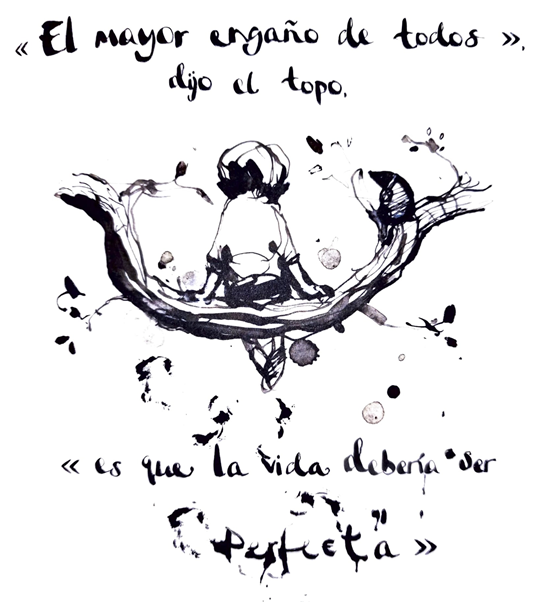
\includegraphics[width=\linewidth]{Fig1.png}
\subcaption{Valores universales: Aceptación.}\label{fig1}
%\source{Autoria própria.}
\end{minipage}
\hfill
\begin{minipage}[t]{0.32\textwidth}
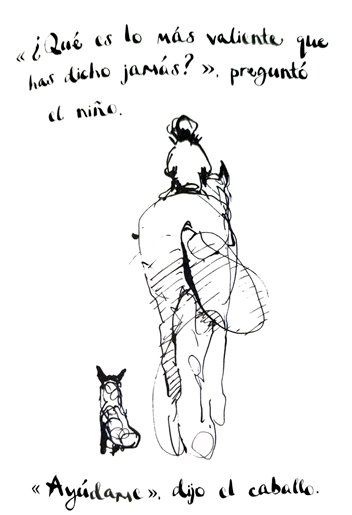
\includegraphics[width=\linewidth]{Fig2.png}
\subcaption{Valores universales: Humildad para pedir ayuda.} \label{fig2}
\end{minipage}
\begin{minipage}[t]{0.32\textwidth}
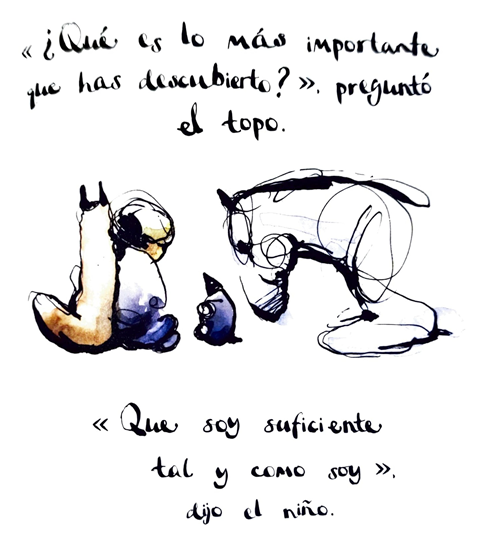
\includegraphics[width=\linewidth]{Fig3.png}
\subcaption{Valores universales: Autoestima.} \label{fig3}
\end{minipage}
\caption{Ilustraciones de \citetitle*{mackesy_nino_2020} \cite{mackesy_nino_2020}.}
\label{fig:01a03}
\source{Versión española del libro.}
\end{figure}



% \begin{figure}[h!]
%  \centering
%  \begin{minipage}[t]{.30\textwidth}
%  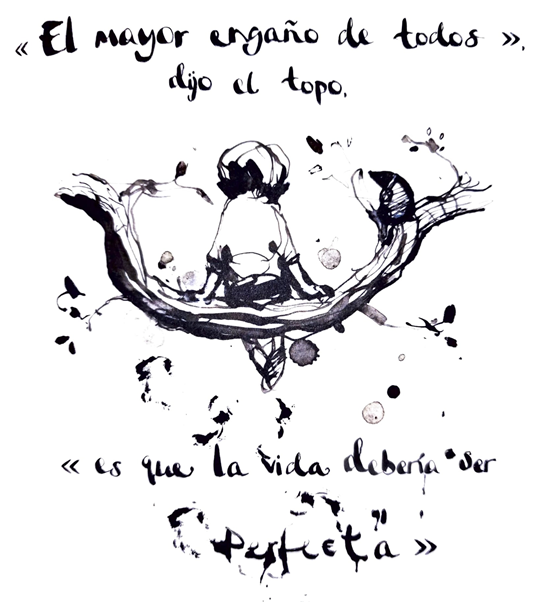
\includegraphics[width=\textwidth]{Fig1.png}
%  \caption{Valores universales: Aceptación.}
%  \label{fig1}
%  %\source{Versión española del libro.}
%  \end{minipage}%
%  \qquad
%  \begin{minipage}[t]{0.30\textwidth}
%  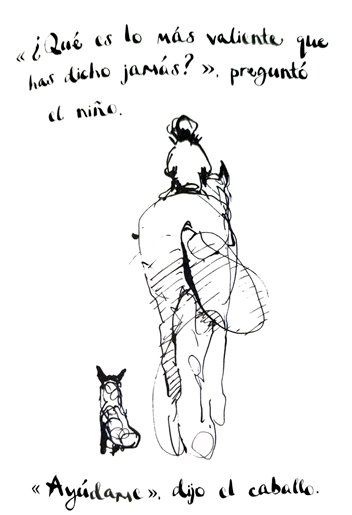
\includegraphics[width=\textwidth]{Fig2.png}
%  \caption{Valores universales: Humildad para pedir ayuda.}
%  \label{fig2}
%  %\source{Versión española del libro.} 
%  \end{minipage}%
%   \qquad
%  \begin{minipage}[t]{0.30\textwidth}
%  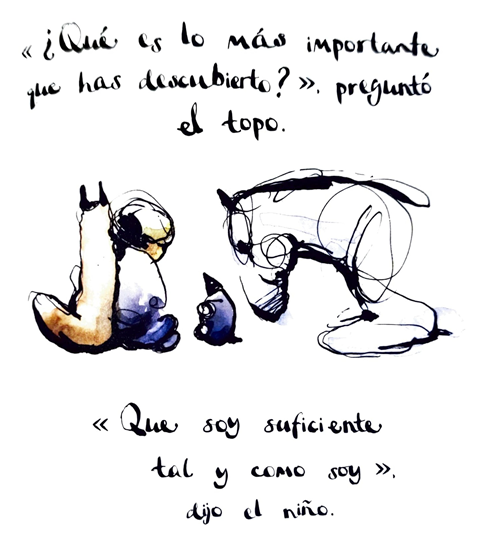
\includegraphics[width=\textwidth]{Fig3.png}
%  \caption{Valores universales: Autoestima.}
%  \label{fig3}
%  %\source{Versión española del libro.} 
%  \end{minipage}%
% \source{Versión española del libro.} 
% \end{figure}



\begin{figure}[htbp]
\centering
\begin{minipage}[t]{0.32\textwidth}
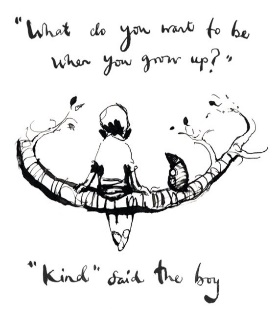
\includegraphics[width=\linewidth]{Fig4.png}
\subcaption{Traduccion al ingles.} \label{fig4}
%\source{Autoria própria.}
\end{minipage}
\hspace{1cm}
\begin{minipage}[t]{0.32\textwidth}
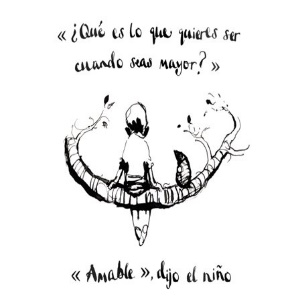
\includegraphics[width=\linewidth]{Fig5.png}
\subcaption{Traduccion al español.} \label{fig5}
\end{minipage}
\\
\begin{minipage}[t]{0.32\textwidth}
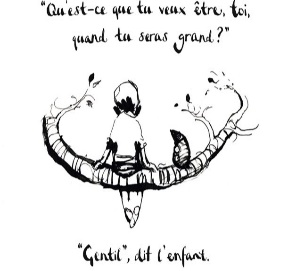
\includegraphics[width=\linewidth]{Fig6.png}
\subcaption{Traduccion al francés.} \label{fig6}
%\source{Autoria própria.}
\end{minipage}
\hspace{1cm}
\begin{minipage}[t]{0.32\textwidth}
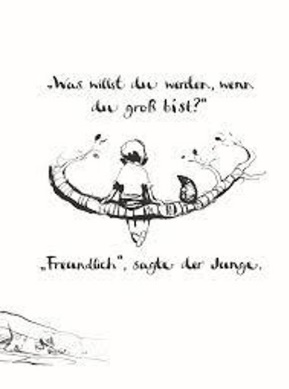
\includegraphics[width=\linewidth]{Fig7.png}
\subcaption{Traduccion al alemán.} \label{fig7}
\end{minipage}

\caption{Versiones del libro en inglés \cite{mackesy_boy_2020a}, español \cite{mackesy_nino_2020}, francés \cite{mackesy_enfant_2020c} y alemán \cite{mackesy_junge_2020d}.}
\label{fig:4a7}
%\source{Caso ambas figuras tenham a mesma autoria, basta especificar a fonte uma única vez.}
\end{figure}


% \begin{figure}[h!]
%  \centering
%  \begin{minipage}[t]{.35\textwidth}
%  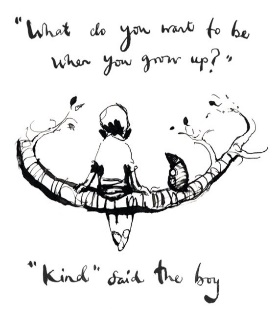
\includegraphics[width=\textwidth]{Fig4.png}
%  \caption{Traduccion al ingles.}
%  \label{fig4}
%  %\source{Versión española del libro.}
%  \end{minipage}%
%  \qquad
%  \begin{minipage}[t]{0.35\textwidth}
%  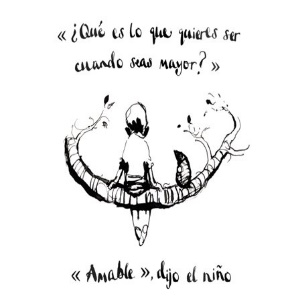
\includegraphics[width=\textwidth]{Fig5.png}
%  \caption{Traduccion al español.}
%  \label{fig5}
%  %\source{Versión española del libro.} 
%  \end{minipage}%
% \end{figure}


% \begin{figure}[h!]
%  \centering
%  \begin{minipage}[t]{0.35\textwidth}
%  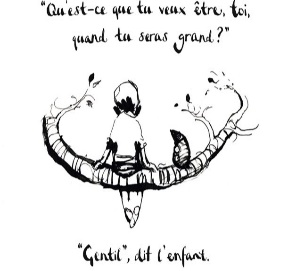
\includegraphics[width=\textwidth]{Fig6.png}
%  \caption{Traduccion al francés.}
%  \label{fig6}
%  %\source{Versión española del libro.} 
%  \end{minipage}%
%    \qquad
%  \begin{minipage}[t]{0.35\textwidth}
%  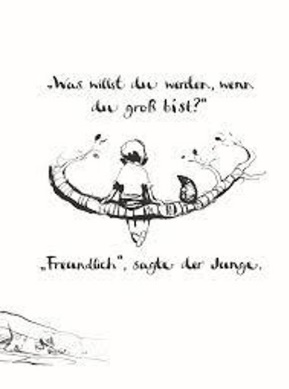
\includegraphics[width=\textwidth]{Fig7.png}
%  \caption{Traduccion al alemán.}
%  \label{fig7}
%  %\source{Versión española del libro.} 
%  \end{minipage}%
% \source{Versiones en diferentes idiomas del libro.} 
% \end{figure}


\section{Conclusiones}\label{sec-organizacao}
En este estudio se ha propuesto una revisión sobre nuevos modelos pedagógicos para la alfabetización adaptada a los actuales contextos educativos condicionados por las tecnologías de la información y de la comunicación, y por la sociedad globalizada que éstas han configurado. Por lo tanto, se hace necesario, reconceptualizar la alfabetización debido a la gran variedad de recursos digitales que emplea diariamente el alumnado en los ámbitos personal y educativo \cite{lopez_pena_propuesta_2022}. Los docentes, por su parte, deben enfrentarse al reto de buscar recursos que se adapten a estos modelos de alfabetización multimodal y plurialfabetización.

La narrativa transmediática y los textos multimodales como el libro ilustrado son excelentes recursos para el desarrollo de la alfabetización en el aula de Educación Primaria. Por otra parte, las recientes políticas de potenciación de lenguas extranjeras en los centros educativos en España favorecen el desarrollo de la plurialfabetización. En este sentido, la traducción de obras de literatura infantil y juvenil a diferentes lenguas constituye un recurso adecuado para implementar esta competencia en el aula.

En este contexto, este estudio ha querido mostrar el potencial pedagógico de un texto transmediático y multimodal en forma de libro ilustrado y su encaje con los enfoques propuestos por los currículos educativos actuales de Educación Primaria.

Estos nuevos modelos de alfabetización suponen para el profesorado un desafío no solo en la búsqueda, adaptación y creación de recursos didácticos, sino también en la exigencia de una actualización de sus competencias docentes. Por otra parte, se necesita investigación sobre la que basar el tratamiento de la multimodalidad en las aulas impulsada por los currículos actuales de enseñanza obligatoria. Aspectos objeto de estudio podrían ser conocer cómo se están llevando a cabo las prácticas con textos multimodales en los distintos niveles educativos o analizar las habilidades que los estudiantes deben adquirir para la producción y recepción de estos.

\printbibliography\label{sec-bib}
% if the text is not in Portuguese, it might be necessary to use the code below instead to print the correct ABNT abbreviations [s.n.], [s.l.]
%\begin{portuguese}
%\printbibliography[title={Bibliography}]
%\end{portuguese}


%full list: conceptualization,datacuration,formalanalysis,funding,investigation,methodology,projadm,resources,software,supervision,validation,visualization,writing,review
\begin{contributors}[sec-contributors]
\authorcontribution{María Victoria López-Pérez}[conceptualization,investigation,supervision,writing,review]
\authorcontribution{María Bobadilla-Pérez}[conceptualization,investigation,writing]
\end{contributors}


\end{document}

